\documentclass[journal,12pt,twocolumn]{IEEEtran}

\usepackage{setspace}
\usepackage{gensymb}
\singlespacing
\usepackage[cmex10]{amsmath}

\usepackage{amsthm}

\usepackage{mathrsfs}
\usepackage{txfonts}
\usepackage{stfloats}
\usepackage{bm}
\usepackage{cite}
\usepackage{cases}
\usepackage{subfig}

\usepackage{longtable}
\usepackage{multirow}
\usepackage{caption}

\usepackage{enumitem}
\usepackage{mathtools}
\usepackage{steinmetz}
\usepackage{tikz}
\usepackage{circuitikz}
\usepackage{verbatim}
\usepackage{tfrupee}
\usepackage[breaklinks=true]{hyperref}
\usepackage{graphicx}
\usepackage{tkz-euclide}
\usepackage{float}
\usepackage[version=4]{mhchem}

\usetikzlibrary{calc,math}
\usepackage{listings}
    \usepackage{color}                                            %%
    \usepackage{array}                                            %%
    \usepackage{longtable}                                        %%
    \usepackage{calc}                                             %%
    \usepackage{multirow}                                         %%
    \usepackage{hhline}                                           %%
    \usepackage{ifthen}                                           %%
    \usepackage{lscape}     
\usepackage{multicol}
\usepackage{chngcntr}

\DeclareMathOperator*{\Res}{Res}

\renewcommand\thesection{\arabic{section}}
\renewcommand\thesubsection{\thesection.\arabic{subsection}}
\renewcommand\thesubsubsection{\thesubsection.\arabic{subsubsection}}

\renewcommand\thesectiondis{\arabic{section}}
\renewcommand\thesubsectiondis{\thesectiondis.\arabic{subsection}}
\renewcommand\thesubsubsectiondis{\thesubsectiondis.\arabic{subsubsection}}


\hyphenation{op-tical net-works semi-conduc-tor}
\def\inputGnumericTable{}                                 %%

\lstset{
%language=C,
frame=single, 
breaklines=true,
columns=fullflexible
}
\begin{document}

\newcommand{\BEQA}{\begin{eqnarray}}
\newcommand{\EEQA}{\end{eqnarray}}
\newcommand{\define}{\stackrel{\triangle}{=}}
\bibliographystyle{IEEEtran}
\raggedbottom
\setlength{\parindent}{0pt}
\providecommand{\mbf}{\mathbf}
\providecommand{\pr}[1]{\ensuremath{\Pr\left(#1\right)}}
\providecommand{\qfunc}[1]{\ensuremath{Q\left(#1\right)}}
\providecommand{\sbrak}[1]{\ensuremath{{}\left[#1\right]}}
\providecommand{\lsbrak}[1]{\ensuremath{{}\left[#1\right.}}
\providecommand{\rsbrak}[1]{\ensuremath{{}\left.#1\right]}}
\providecommand{\brak}[1]{\ensuremath{\left(#1\right)}}
\providecommand{\lbrak}[1]{\ensuremath{\left(#1\right.}}
\providecommand{\rbrak}[1]{\ensuremath{\left.#1\right)}}
\providecommand{\cbrak}[1]{\ensuremath{\left\{#1\right\}}}
\providecommand{\lcbrak}[1]{\ensuremath{\left\{#1\right.}}
\providecommand{\rcbrak}[1]{\ensuremath{\left.#1\right\}}}
\theoremstyle{remark}
\newtheorem{rem}{Remark}
\newcommand{\sgn}{\mathop{\mathrm{sgn}}}
\providecommand{\abs}[1]{\vert#1\vert}
\providecommand{\res}[1]{\Res\displaylimits_{#1}} 
\providecommand{\norm}[1]{\lVert#1\rVert}
%\providecommand{\norm}[1]{\lVert#1\rVert}
\providecommand{\mtx}[1]{\mathbf{#1}}
\providecommand{\mean}[1]{E[ #1 ]}
\providecommand{\fourier}{\overset{\mathcal{F}}{ \rightleftharpoons}}
%\providecommand{\hilbert}{\overset{\mathcal{H}}{ \rightleftharpoons}}
\providecommand{\system}{\overset{\mathcal{H}}{ \longleftrightarrow}}

	%\newcommand{\solution}[2]{\textbf{Solution:}{#1}}
\newcommand{\solution}{\noindent \textbf{Solution: }}
\newcommand{\cosec}{\,\text{cosec}\,}
\providecommand{\dec}[2]{\ensuremath{\overset{#1}{\underset{#2}{\gtrless}}}}
\newcommand{\myvec}[1]{\ensuremath{\begin{pmatrix}#1\end{pmatrix}}}
\newcommand{\mydet}[1]{\ensuremath{\begin{vmatrix}#1\end{vmatrix}}}
\newcommand\comb[2][^n]{\prescript{#1\mkern-0.5mu}{}C_{#2}}

\numberwithin{equation}{subsection}
\makeatletter
\@addtoreset{figure}{problem}
\makeatother
\let\StandardTheFigure\thefigure
\let\vec\mathbf
\renewcommand{\thefigure}{\theproblem}
\def\putbox#1#2#3{\makebox[0in][l]{\makebox[#1][l]{}\raisebox{\baselineskip}[0in][0in]{\raisebox{#2}[0in][0in]{#3}}}}
     \def\rightbox#1{\makebox[0in][r]{#1}}
     \def\centbox#1{\makebox[0in]{#1}}
     \def\topbox#1{\raisebox{-\baselineskip}[0in][0in]{#1}}
     \def\midbox#1{\raisebox{-0.5\baselineskip}[0in][0in]{#1}}
\vspace{3cm}

\title{AI1103-Assignment-5}
\author{Name: Vikhyath Sai Kothamasu\\Roll Number: CS20BTECH11056}
\maketitle
\newpage
\bigskip
\renewcommand{\thefigure}{\theenumi}
\renewcommand{\thetable}{\theenumi}

\begin{figure} [h]
    \includegraphics[width = 0.8\columnwidth]{college logo.png}
\end{figure}

Download all python codes from 
\begin{lstlisting}
https://github.com/Vikhyath-vec/AI1103/tree/main/Assignment-5/codes
\end{lstlisting}
%
and latex-tikz codes from 
%
\begin{lstlisting}

https://github.com/Vikhyath-vec/AI1103/blob/main/Assignment-5/Assignment-5.tex
\end{lstlisting}
\section*{Question}

Let $X$ be the number of heads in 4 tosses of a fair coin by Person 1 and let $Y$ be the number of heads in 4 tosses of a fair coin by Person 2. Assume that all the tosses are independent. Then the value of $\mathbb{P}(X=Y)$ correct up to three decimal places is $\rule{1.6cm}{0.15mm}$ .

\section*{Solution}
Let $X \in \{ 0, 1, 2, 3, 4\}$ be the random variable representing the number of heads obtained by Person 1 in 4 tosses. Similarly, Let $Y \in \{ 0, 1, 2, 3, 4\}$ be the random variable representing the number of heads obtained by Person 2 in 4 tosses. Then $X \text{ and } Y$ are binomial distributions with parameter:
\begin{align}
    p = \frac{1}{2}
\end{align}
Then,
\begin{align}
    \Pr(X=i) = 
	\begin{cases}
	\comb[4]{k}(p)^k(1-p)^{4-k} &  i \in \{0, 1, 2, 3, 4\}\\ ~\\[-1em]
	0 & \text{otherwise}
	\end{cases}
	\\\Pr(X=i) = 
	\begin{cases}
	\comb[4]{k}(\frac{1}{2})^k(1-\frac{1}{2})^{4-k}  &  i \in \{0, 1, 2, 3, 4\}\\ ~\\[-1em]
	0 & \text{otherwise}
	\end{cases}
	\\\Pr(X=i) = 
	\begin{cases}
	\comb[4]{k}\times(\frac{1}{2})^4  &  i \in \{0, 1, 2, 3, 4\}\\ ~\\[-1em]
	0 & \text{otherwise}
	\end{cases}
\end{align}
\begin{center}
\begin{table}[h]
    \centering
    \resizebox{\columnwidth}{!}{
\begin{tabular}{|c|c|c|}
\hline
Serial number & Case & Probability of the case \\
\hline
1 & $\Pr(X=0)$ & $\frac{\comb[4]{0}}{16} = \frac{1}{16}$ \\ 
\hline
2 & $\Pr(X=1)$ & $\frac{\comb[4]{1}}{16} = \frac{4}{16}$ \\ 
\hline
3 & $\Pr(X=2)$ & $\frac{\comb[4]{2}}{16} = \frac{6}{16}$ \\
\hline
4 & $\Pr(X=3)$ & $\frac{\comb[4]{3}}{16} = \frac{4}{16}$ \\
\hline
5 & $\Pr(X=4)$ & $\frac{\comb[4]{4}}{16} = \frac{1}{16}$ \\
\hline
\end{tabular}
}
    \caption{Probability distribution table of X}
    \label{table 1}
\end{table}
\end{center}
Similar is the distribution of $Y$. For finding $\Pr{(X=Y)}$, let $Y=y$,
\begin{align}
    \Pr{(X=Y=y)} = \frac{\comb[4]{y}}{16} \times \Pr{(Y=y)}
\end{align}
Generalizing this result,
\begin{align}
    \Pr{(X=Y)} &= \sum_{y=0}^4  \frac{\comb[4]{y}}{16}\times \Pr{(Y=y)}
    \\ &= \sum_{y=0}^4 \frac{\comb[4]{y}}{16} \times \frac{\comb[4]{y}}{16}
\end{align}
\begin{multline}
    \Pr{(X=Y)} = \brak{\frac{1}{16}\times\frac{1}{16}} + \brak{\frac{4}{16}\times\frac{4}{16}} +\brak{\frac{6}{16}\times\frac{6}{16}} \\+\brak{\frac{4}{16}\times\frac{4}{16}} +\brak{\frac{1}{16}\times\frac{1}{16}} 
\end{multline}
\begin{align}
    \Pr{(X=Y)} &= \frac{1}{256} + \frac{16}{256} +\frac{36}{256} +\frac{16}{256} +\frac{1}{256} 
    \\&= \frac{70}{256} 
    \\&= \frac{35}{128} 
    \\&= 0.2734375
\end{align}
The the value of $\mathbb{P}(X=Y)$ correct up to three decimal places is 0.273.
\begin{figure} [H]
    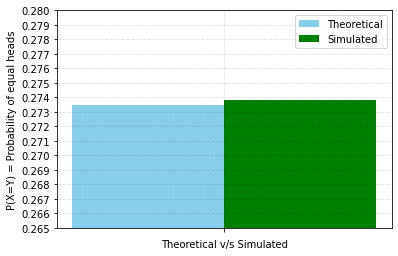
\includegraphics[width = 0.9\columnwidth]{graph.png}
    \caption{Theoretical and simulated results}
    \label{Fig 1}
\end{figure}
\end{document}
